\section{Assembly component}

\textbf{Created by:} Dušan Šormaz \\
\textbf{Modified by:}  \\

address all times/ sometimes and also transitivity of these two pairs of relationships.

\subsection*{Scenario Objective}
From Arko's email, 1/7/25 
I want to mention that however we are showing the basic use of "component part of" relation for expressing parthood, we should also show the use of "at some time" vs. "at all times" under this scenario. Also, the nuanced semantics of "component of at all times" vs. "has component at all times" (explain why they are not inverses to each other) is to be examined.
DNS
We also need to show multiple levels of assemblies, at least three. Should we consider assembly process(es)?
\subsection*{General Pattern Description}
This scenario shows uses of \texttt{iof:componetPartOf}, \texttt{bfo:continuantPartofAtSomeTime}, and \texttt{bfo:continuantPartofAtAllTimes} object properties. The general pattern is shown in fig. 

\begin{figure}
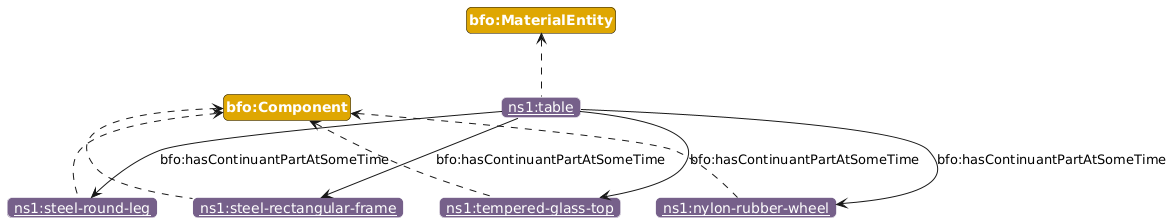
\includegraphics[scale=0.5]{scenarios/object-artifact-material/image/what-is-made-of.png}
\caption{The general pattern for the use of component related object properties} 
\label{gen-pttn-components}
\end{figure}


\subsection*{Examples}

A car engine is often showcased in parts: pistons, crankshaft, and cylinders.

An insulated wall comprises drywall, insulation foam, and outer sheathing.

Sewing patches of silk, cotton and leather make an item of clothing.

\section{Embedded components}

Reinforcement Bars in Concrete Structures

coating on a metal surface - this is not assembly

printed circuit on board

Embedded sensors